\documentclass[tikz]{standalone}

\usepackage{pgfplots}
\pgfplotsset{compat=1.15}

\usepackage{pgfplots}


%\newcommand\HUGE{\@setfontsize\Huge{48}{57}} 
\makeatletter
\newcommand\HUGE{\@setfontsize\Huge{90}{100}}
\makeatother   
\makeatletter
\newcommand\hugest{\@setfontsize\Huge{110}{120}}
\makeatother   
\begin{document}
\begin{tikzpicture}[scale=1]
\node at (-4,0)
    {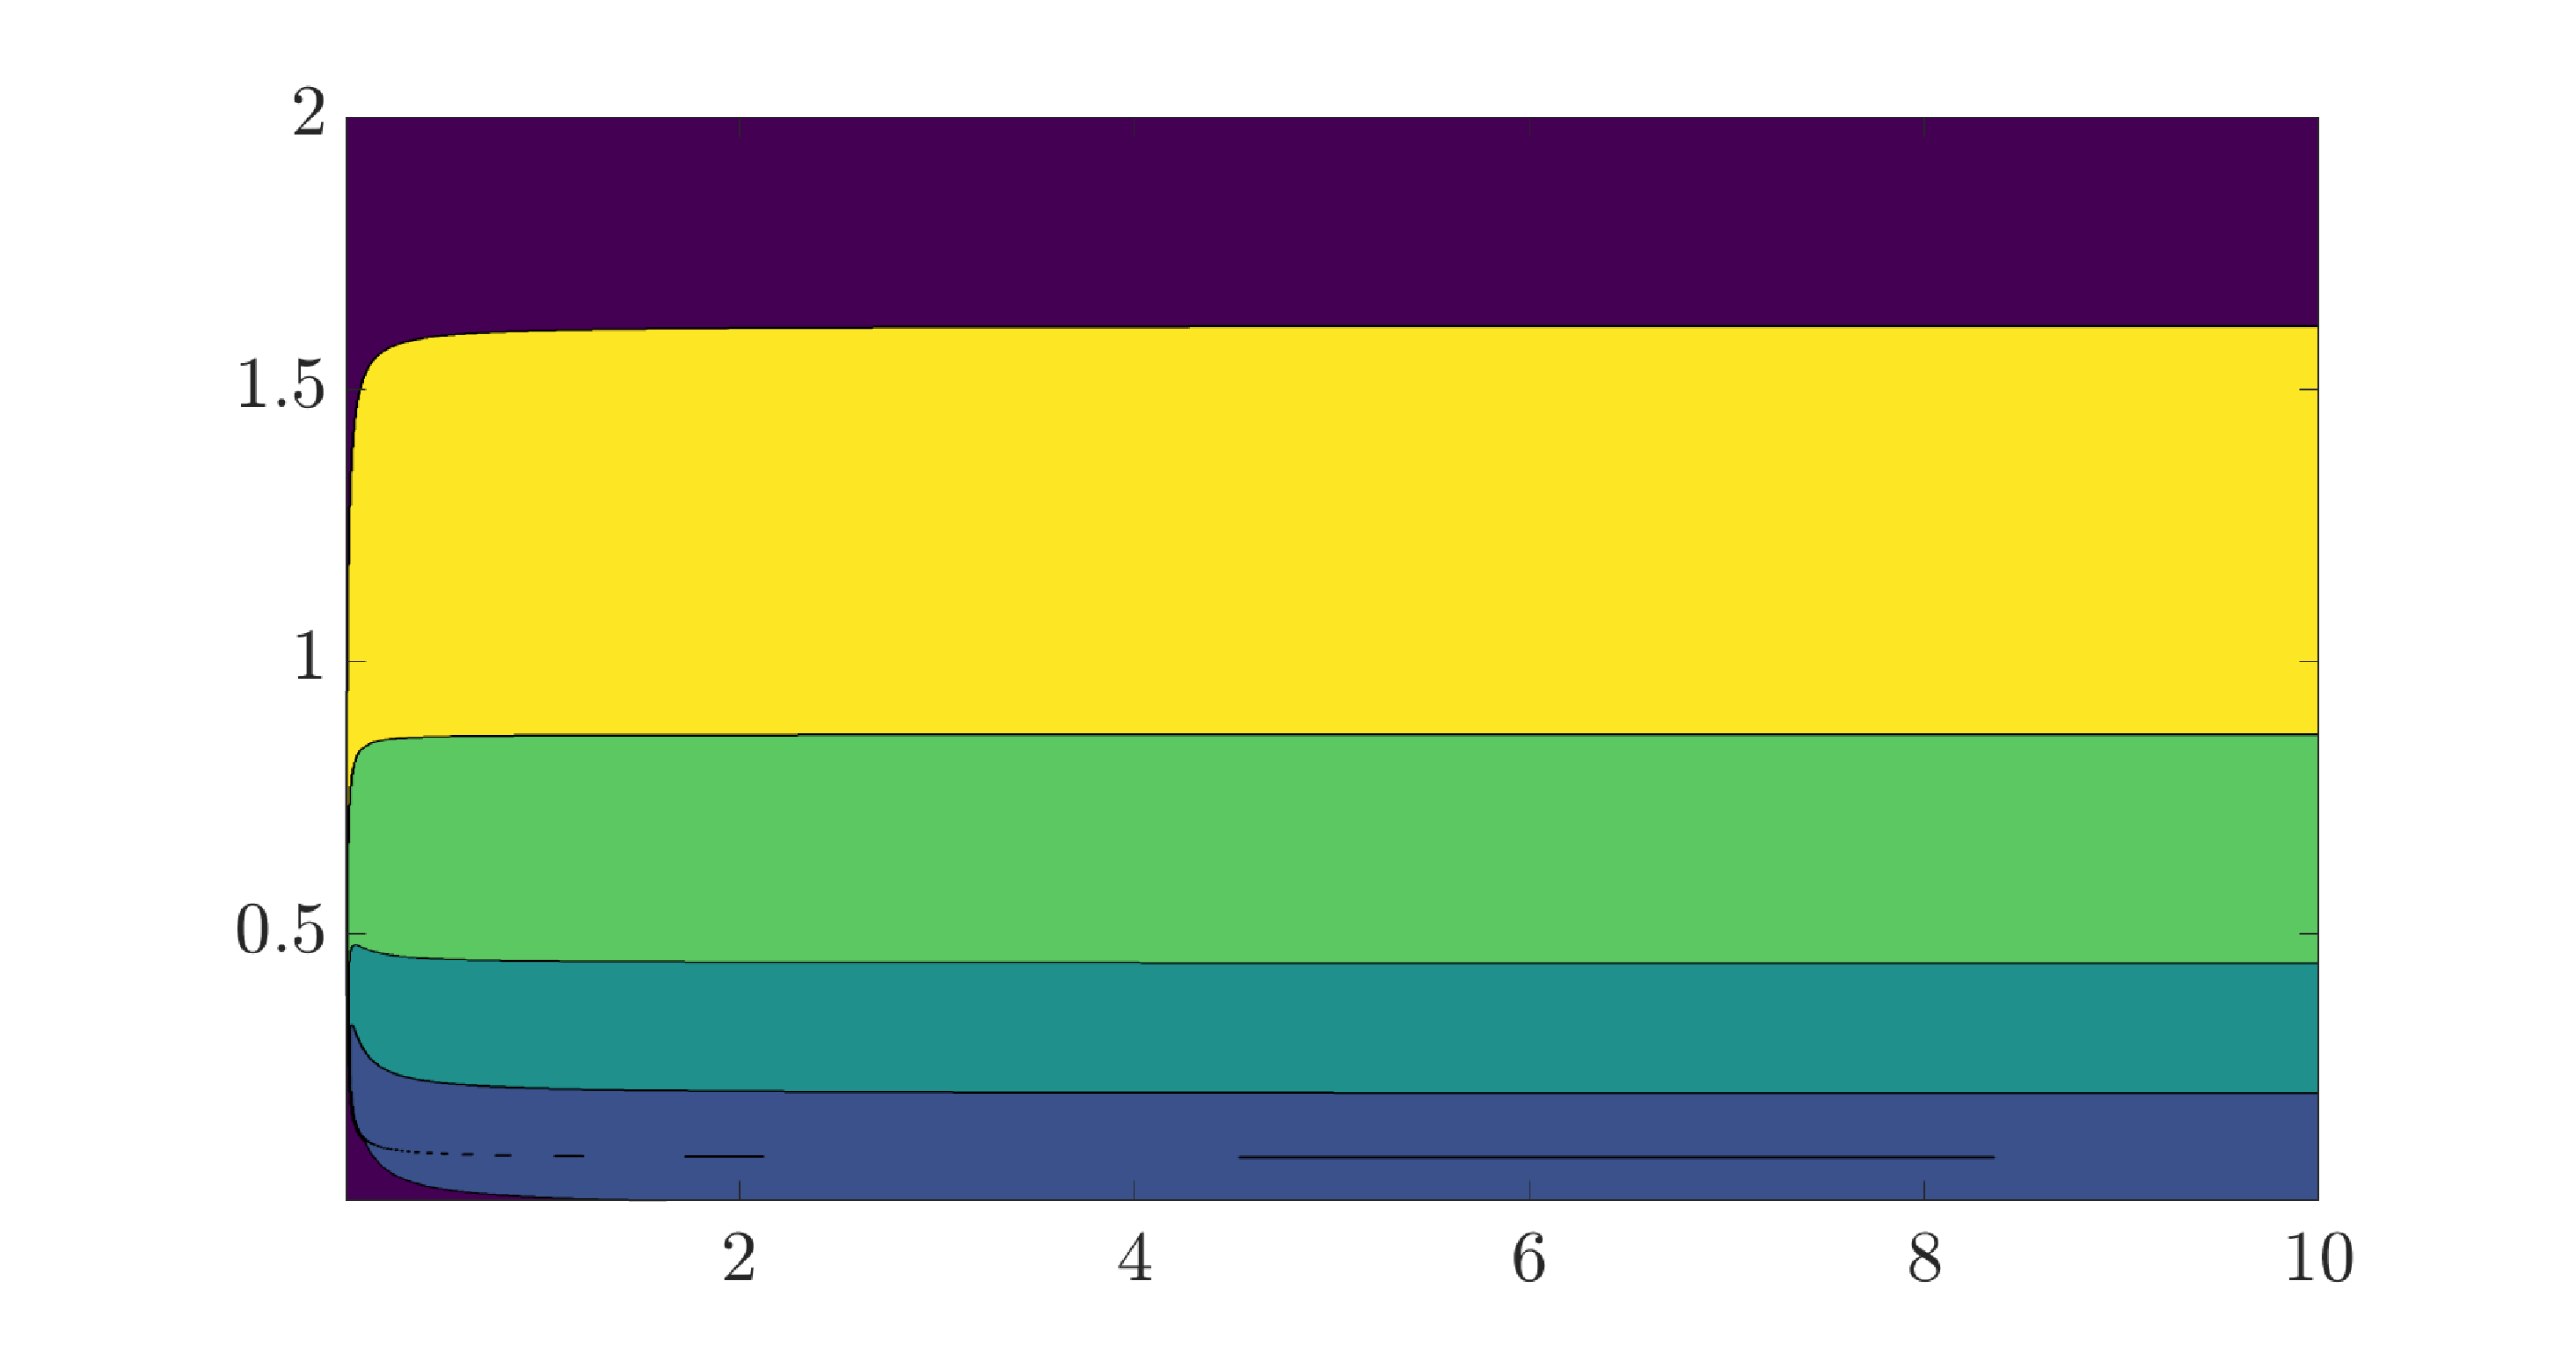
\includegraphics[scale=0.5]{./c1VSc2.eps}};    
    \node at (-26.5,0)
    {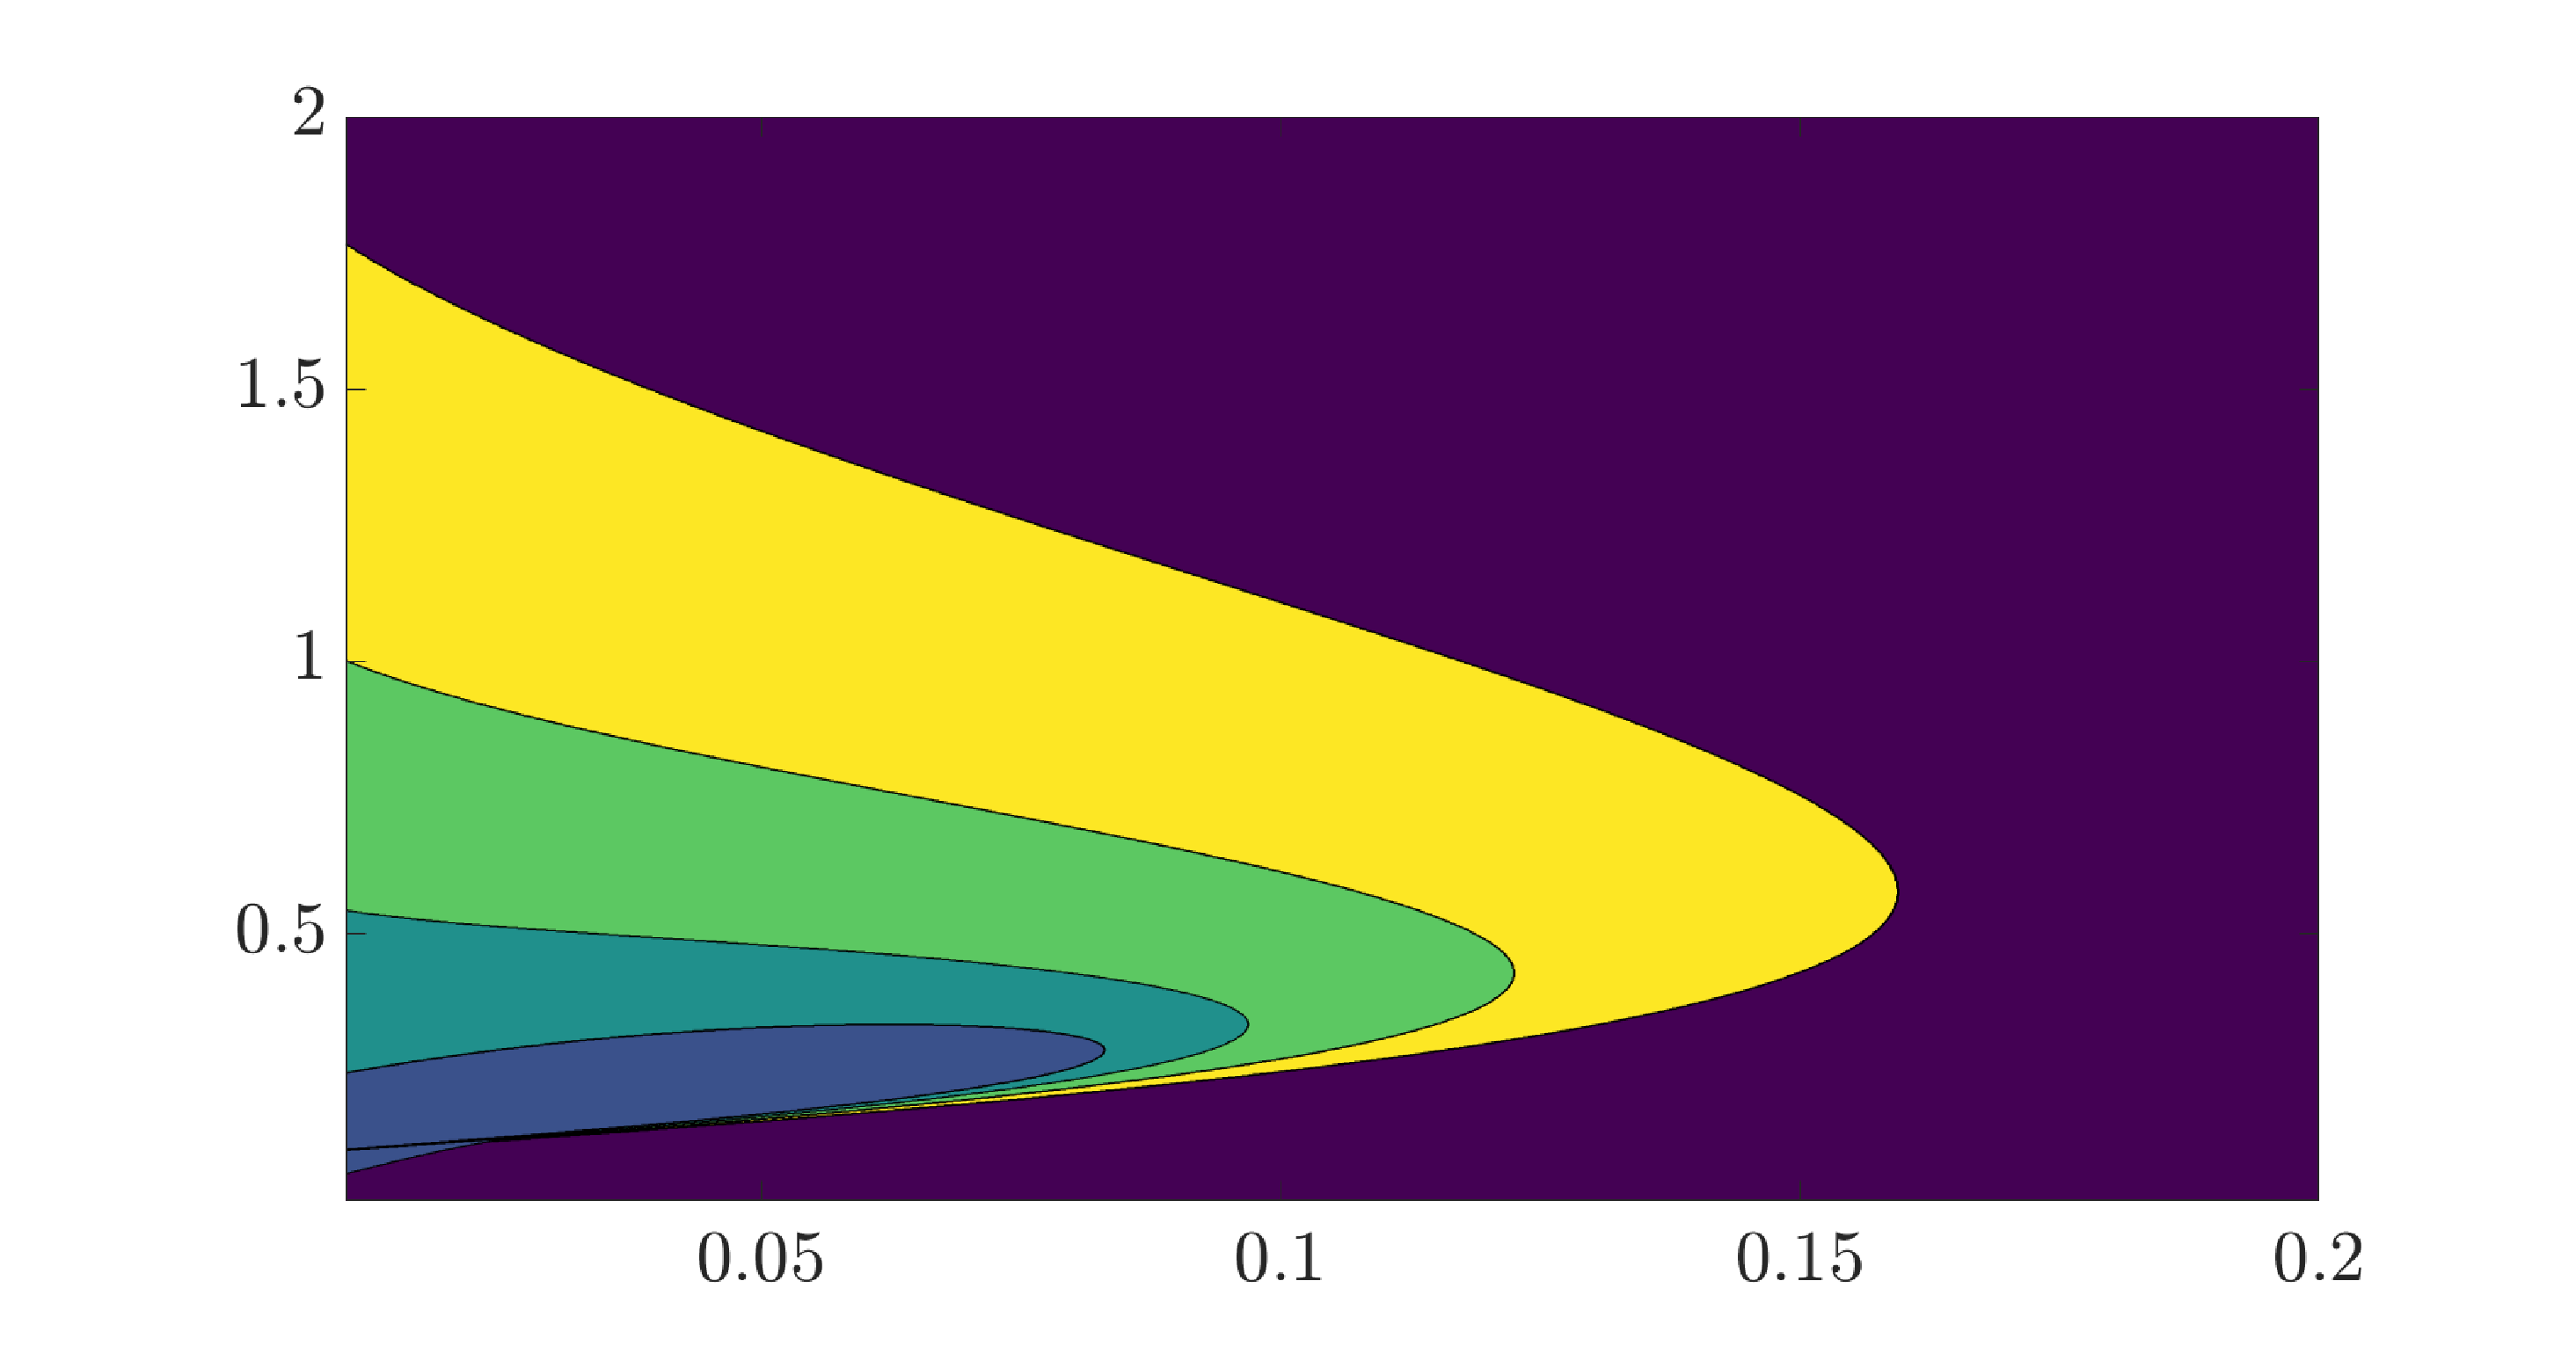
\includegraphics[scale=0.5]{./c_1VSc2.eps}};        
\begin{axis}[
 colormap={example}{ samples of colormap=(6 of viridis) }, 
 colorbar, 
 colorbar sampled, 
 colorbar/width=7mm,
    colorbar style = {
	     at={(1.00,0.96)},
    	ylabel= {} ,
	ylabel style = { at={(3.0,0.35)},
	rotate = 180},
	yticklabel pos =left,
	ymax =1.0,
	ymin = 0,	
	yticklabels = {{},{},{},{},{}},
	ytick={0,0.25, 0.5, 0.75,1},		
	height = 103.5mm,
	samples=6
    },
%colorbar style={samples=4}, 
 colormap access=piecewise const,
       axis line style={draw=none},
      tick style={draw=none},
       yticklabels={,,,,},      
	xticklabels={,,,,},
] 

\end{axis}    
%=========================================================
% TO MAKE SURE EVERYTHING IS IN LINE: UNCOMMENT TO SEE
%\draw [-,line width=0.5mm] (-40,5.5) -- (10,5.5);
%\draw [-,line width=0.5mm] (-40,-4.90) -- (10,-4.90);
%\draw [-,line width=0.5mm] (-40,-4.90) -- (10,-4.90);
%=========================================================
% THE AXES LABELS
\node[align=center,rotate=90] at (-38,0.18) {\huge Dimensionless rate of activation, $c_2$:\\ \huge $\textrm{Cdc42-GDP}\longrightarrow\textrm{Cdc42-GTP}$};
\node[align=center] at (-3.5,-7.2) {\huge Dimensionless rate of cytosolic flux to the membrane, $c_{1}$:\\ \huge $\textrm{Cdc42-GDI}\longrightarrow\textrm{Cdc42-GDP}$\\\large};
\node[align=center] at (-26.25,-7.2) {\huge Dimensionless rate of dissociation from the membrane, $c_{-1}$:\\ \huge $\textrm{Cdc42-GDP}\longrightarrow\textrm{Cdc42-GDI}$\\\huge};
% THE LABELS FOR THE COLOURBAR
\node[align=center] at (9.05,4.2) {\huge Classic\\\huge $d=30$};
\node[align=center] at (9.05,2.2) {\huge Classic\\\huge $d=10$};
\node[align=center] at (9.05,0.0) {\huge Classic\\\huge $d=5$};
\node[align=center] at (9.35,-2.0) {\huge Non-classic};
\node[align=center] at (9.5,-4) {\huge No\\\huge Symmetry\\\huge Breaking};
% A and B panels
\node[align=center] at (-35,6.5) {\HUGE \textbf{(A)}};
\node[align=center] at (-12.5,6.5) {\HUGE \textbf{(B)}};
\end{tikzpicture}
\end{document}